\section{Thornton and Marion Problem 10.1}
Calculate the centrifugal acceleration, due to Earth's rotation, on a particle on the surface of Earth at the equator. Compare this result with the gravitational acceleration. Compute also the centrifugal acceleration due to the motion of Earth about the Sun and justify the remark made in the text that this acceleration may be neglected compared with the acceleration caused by the axial rotation.

\subsection{Part 1}
Suppose Earth is rotating around it's principal axis with angular velocity $\omega$ and has a radius $R$. Then the centrifugal acceleration of a particle at the equator with mass $m$ is

\begin{equation}
    \begin{split}
        F_{cent} &= -m \omega \times (\omega \times r)\\
        F_{cent} &= m\omega^2R \textrm{ since $\omega$ is normal to $R$}
    \end{split}
\end{equation}

So the centrifugal and gravitational acceleration are

\begin{equation}
    \begin{split}
        a_{cent} &= \omega^2R\\
        &= (\SI{7.292115}{\frac{\radian}{\second}})^2(\SI{6378e3}{\meter}) \approx \SI{0.03391}{\frac{\meter}{\second^2}}\\
        a_{grav} &= G\frac{M}{R^2}\\
        &= \SI{6.67408e-11}{\frac{\newton\meter^2}{\kilo\gram^2}}\frac{\SI{5.972e24}{\kilo\gram}}{(\SI{6378e3}{\meter})^2} \approx \SI{9.798}{\frac{\meter}{\second^2}}
    \end{split}
\end{equation}

Comparing

\begin{equation}
    \begin{split}
        \frac{a_{grav}}{a_{cent}} &= \frac{GM}{\omega^2R^3}\\
        \frac{a_{grav}}{a_{cent}} &= \frac{(\SI{6.67408e-11}{\frac{\newton\meter^2}{\kilo\gram^2}})(\SI{5.972e24}{\kilo\gram})}{(\SI{7.292115}{\frac{\radian}{\second}})^2(\SI{6378e3}{\meter})^3} \approx 288.9
    \end{split}
\end{equation}

\subsection{Part 2}
Suppose the Earth moves around the Sun in a circular orbit with radius $R'$ and angular velocity $\omega'$. Then the centrifugal acceleration is

\begin{equation}
\begin{split}
    a_{cent} &= \omega'^2R'\\
    &= (\frac{2\pi}{\SI{365.256}{\day}}\frac{\SI{1}{\day}}{\SI{86400}{\second}})^2(\SI{149.60e9}{\meter})\\
    &= \approx \SI{5.9302e-3}{\frac{\meter}{\second^2}}
\end{split}
\end{equation}

\section{Thornton and Marion Problem 10.4}
In Example 10.2, for what initial velocity and direction in the rotating system will the hockey puck appear to be subsequently motionless in the fixed system? What will be the motion in the rotating system? Let the initial position be the same as in Example 10.2. You may choose to do a numerical calculation.
\begin{figure}[h]
    \centering
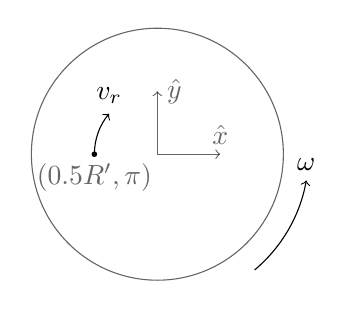
\begin{tikzpicture}[scale=1.6]
    \coordinate (origin) at (0,0);
    \coordinate (init) at (180:0.5);
    \coordinate (ref) at (160:0.5);

    \draw[opacity=0.6] (origin) circle (1);


    \draw[->,opacity=0.6] (origin) -- (0:0.5) node[above] {$\hat{x}$};

    \draw[->,opacity=0.6] (origin) -- (90:0.5) node[right] {$\hat{y}$};

    \draw[fill=black] (init) circle (0.5pt);

    \node[below,opacity=0.6] (point) at (init) {$(0.5R',\pi)$};

    \draw[->] (init) arc (180:140:0.5cm) node[above] {$v_r$};

    \draw[->] (-50:1.2) arc (-50:-10:1.2) node[above] {$\omega$};
    
\end{tikzpicture}
\end{figure}
\subsection{Part 1}
In polar coordinates the starting position is $(0.5R,\pi)$. Starting with
\begin{equation}
    v_f = V + v_r + \omega \times r\\
\end{equation}
By construction $v_f = V = 0$. So (5.1) becomes
\begin{equation}
\begin{split}
    0 &= \dot{R}\hat{r} +\dot{\theta} R\hat{\theta} + \omega \hat{z} \times R\hat{r}\\
    0& = \dot{R}\hat{r} +\dot{\theta} R\hat{\theta} + \omega R\hat{\theta}
\end{split}
\end{equation}
It follows that $\dot{\theta} = -\omega \textrm{ and } \dot{R} = 0$. So the initial velocity in polar coordinates is
\begin{equation}
\begin{split}
    v_r(0) = (0, -\omega)
\end{split}
\end{equation}
In Cartesian coordinates
\begin{equation}
    \begin{split}
        v_f &= \begin{bmatrix}
\dot{R}\cos(\theta) - R \dot{\theta} \sin(\theta) \\
\dot{R}\sin(\theta) + R \dot{\theta} \cos(\theta) 
\end{bmatrix}\\
        v_f(0) &= -\frac{\omega}{2}R' \begin{bmatrix}
0 \\
-1 
\end{bmatrix}= (0,\frac{1}{2}R'\omega)\\
    \end{split}
\end{equation}

\subsection{Part 2}
In the rotating system, from (5.2)
\begin{equation}
    \begin{split}
        \theta(t) &= \pi - \omega t \mod 2\pi\\
        R(t) &= R(0) = \frac{1}{2}R'
    \end{split}
\end{equation}
The hockey puck moves with a fixed radius from the axis of rotation, $R(0)$, and a constant angular velocity $-\omega$.

\section{Accelerating Wave Potential}

\subsection{Part 1}
If $kV_0 = 2ma_f$ then the $\sin$ wave fixed points are
\begin{equation}
\begin{split}
    \frac{d\widetilde{p}}{dt} = -\partial_x V &= -2ma_f \sin(k \widetilde{x}) = 0\\
    \implies \widetilde{x} &= \frac{n\pi}{k}
\end{split}
\end{equation}

\subsection{Part 2}
If $kV_0 = 2ma_f$ then the triangle wave fixed points are
\begin{equation}
    \begin{split}
        \frac{d\widetilde{p}}{dt} = -\partial_x V&= -2kma_f \widetilde{x} = 0\\
        \implies \widetilde{x} &= 0
    \end{split}
\end{equation}
The stable points are at
\begin{equation}
    \begin{split}
        -\partial_x \frac{d\widetilde{p}}{dt}|_{\widetilde{x} =0} &= -\frac{\partial \widetilde{x}}{\partial x} \partial_{\widetilde{x}} (-2kma_f \widetilde{x})|_{\widetilde{x} =0}\\
        & = 2kma_f\\
        & = k^2 V_0 > 0\\
        \implies \widetilde{x} &= 0 \textrm{ is stable}
    \end{split}
\end{equation}

\subsection{Part 3}
Taylor expanding $U(\widetilde{x})$ at $0$
\begin{equation}
    \begin{split}
        U(\widetilde{x}) &= U(0) - \frac{d\widetilde{p}}{dt} - \frac{1}{2!}\frac{d^2}{d\widetilde{x}dt}\widetilde{x} - \frac{1}{3!}\frac{d^2}{d\widetilde{x}^2dt}\widetilde{x}^2 + \dots\\
         &= U(0)+kma_f
    \end{split}
\end{equation}

\section{Yo-yo}

\subsection{Part 1}
Suppose that the string takes up no space. After the center of the yo-yo has fallen $x$ meters it has rotated $\theta = \frac{2}{a}x$ radians.
\begin{equation}
    \frac{dh}{dt} = v_{com} = \frac{a}{2}\omega
\end{equation}
The gravitational potential energy is
\begin{equation}
    U = -mgx
\end{equation}
The kinetic energy is
\begin{equation}
\begin{split}
    T &= T_{trans} + T_{rot}\\
    &= \frac{1}{2}mv_{com}^2+\frac{1}{2}I_c\omega^2\\
    &= \frac{3}{2}mv_{com}^2
\end{split}
\end{equation}
The Lagrangian is
\begin{equation}
    \begin{split}
        L &= \frac{3}{2}mv_{com}^2+mgx\\
        L_x &= mg \textrm{ and } \partial_t L_{\dot{v}_{com}} = 3m\dot{v}_{com}\\
    \end{split}
\end{equation}
Then the equation of motion and final velocities are
\begin{equation}
    \begin{split}
        x(t) &= \frac{gt^2}{6}\\
        v(L) &= \sqrt{\frac{2}{3}gL}\\
       \omega(L) &= \sqrt{\frac{8}{3}\frac{gL}{a^2}}
    \end{split}
\end{equation}

\subsection{Part 2}
Assume that the distance between the bottom of the string and the top of the quarter cylinder is negligible.

The total energy at the top of the quarter circle is
\begin{equation}
    \begin{split}
        E_{Total} &= U + T_{Trans} + T_{Rot}\\
        &= mgc + \frac{1}{2}m\dot{y}_i^2 + \frac{1}{2}I\omega_i^2\\
    \end{split}
\end{equation}
The energy at the bottom of the quarter circle is
\begin{equation}
    \begin{split}
        E_{Total} &= T_{Trans} + T_{Rot}\\
        &= \frac{1}{2}m\dot{x}_f^2 + \frac{1}{2}I\omega_f^2
    \end{split}
\end{equation}
Since the ramp is friction-less the torque about the center of mass from the normal and gravitational force is $0$, so $\omega_i = \omega_f$. The torque about the point of contact with the quarter circle will change the linear momentum. By conservation of energy then
\begin{equation}
\begin{split}
    \frac{1}{2}m\dot{x}_f^2 &= mgc + \frac{1}{2}m\dot{y}_i^2\\
    \dot{x}_f &= \sqrt{2gc + \dot{y}_i^2}\\
    v &= \sqrt{2gc+\frac{2}{3}gL}\\
    \omega_f &= \sqrt{\frac{8}{3}\frac{gL}{a^2}}
\end{split}
\end{equation}

\subsection{Part 3}
Let $\mu$ be the coefficient of static friction and assume there is no rolling resistance. The normal force and gravitational force provide no torque. The friction force will oppose the transnational motion and provide a torque
\begin{equation}
\begin{split}
    m\ddot{x} &= -\mu mg\\
    \dot{x}(t) &= -\mu g t + \dot{x}(0)\\
    \tau &= -\mu mg a = I\dot{\omega}\\
    \omega &= \omega(0)-\frac{\mu g}{2a}t
\end{split}
\end{equation}
Rolling without slipping occurs when $\dot{x} = a \omega$, so
\begin{equation}
\begin{split}
    -\mu gt+\dot{x}(0) &= a\omega(0) -\frac{1}{2}\mu g t\\
    \frac{1}{2}\mu g t &= a\omega(0)-\dot{x}(0)\\
    t &= \frac{2a}{\mu g}\omega(0)-\frac{2}{\mu g}\dot{x}(0)\\
\end{split}
\end{equation}
Plugging the time back into (5.9)
\begin{equation}
    \begin{split}
        \dot{x} & = - 2a \omega(0) + 3\dot{x}(0)\\
        \dot{x} &=-2a\sqrt{\frac{8}{3}\frac{gL}{a^2}}+3\sqrt{2gc+\frac{2}{3}gL}\\
        \omega &= \frac{1}{a}\dot{x}(0)\\
        \omega &= \frac{1}{a}\sqrt{2gc+\frac{2}{3}gL}
    \end{split}
\end{equation}

\section{Thornton and Marion Problem 11.2}
Calculate the moments of inertia $I_1, I_2,$ and $I_3$ for a homogeneous cone of mass $M$ whose height is $h$ and whose base has a radius $R$. Choose the $x_3-$axis along the axis of symmetry of the cone. Choose the origin at the apex of the cone, and calculate the elements of the inertia tensor. Then make a transformation such that the center of mass of the cone becomes the origin, and find the principal moments of inertia.
\pgfplotsset{colormap={CM}{rgb=(0,0,1) color=(black) rgb255=(238,140,238)}}

\begin{figure}[h]
    \centering
\begin{tikzpicture}

    \begin{axis}[
    hide axis,
    view={120}{30},
      xmin=-1.5,
      xmax=1.5,
      ymin=-1.5,
      ymax=1.5,
      zmin=0,
      zmax = 2,
]

% Parametric equations for the cone
\addplot3[
    surf,
    colormap/bone,
    faceted color=none,
    domain=0:360,
    variable = t,
    y domain=0:1,
    variable y = r,
    samples=30,
    samples y=20,
] ({r*sin(t)}, {r*cos(t)}, {r*2});

% Draw unit vectors for x, y, z axes
% Draw unit vectors for x, y, z axes
\draw[->] (axis cs:0,0,0) -- (axis cs:1,0,0) node[pos=1.2]{$x_1$};
\draw[->] (axis cs:0,0,0) -- (axis cs:0,1,0) node[pos=1.2]{$x_2$};
\draw[->,opacity=0.5] (axis cs:0,0,0) -- (axis cs:0,0,2) node[pos=1.1, opacity=1]{$x_3$};

\draw[dashed] (axis cs:0,0,2)-- node[above] {$R$} (axis cs:0,1,2);
\draw[dashed] (axis cs:0,1,0) -- node[right] {$h$} (axis cs: 0,1,2);
    \end{axis}

\end{tikzpicture}
\end{figure}

\subsection{Part 1}
Starting with
\begin{equation}
\begin{split}
    I =\int_V \rho(r)(I |r|^2-rr^T) dv \textrm{ and } \rho = \frac{3M}{\pi R^2 h}\\
\end{split}
\end{equation}
By symmetry and constant density
\begin{equation}
\begin{split}
    I_{1,2} &= \rho \int_V (x_{2}^2+x_3^2)dV\\
    &= \rho \int_0^h \int_0^{\frac{R}{h}z} \int_0^{2\pi} (r^2\sin^2\theta + z^2) r d\theta dr dz\\
    &=\rho \int_0^h \int_0^{\frac{R}{h}z}r^3drdz\int_0^{2\pi}\sin^2\theta d\theta + \rho \int_0^{2\pi} \int_0^h z^2 \int_0^{\frac{R}{h}z}rdrdz\\
    &=\rho \frac{1}{20}\pi R^4 h + \rho\frac{1}{5}\pi R^2 h^3\\
    &= \frac{3M}{20}R^2+\frac{3M}{5}h^2
\end{split}
\end{equation}
For the $x_3$ axis
\begin{equation}
\begin{split}
    I_{3} &= \rho \int_V (x_2^2+x_1^2)dV\\
&= \rho \int_0^h \int_0^{\frac{R}{h}z} \int_0^{2\pi} (r^2\sin^2\theta + r^2\cos^2\theta) r d\theta dr dz\\
&=\rho \int_0^h \int_0^{\frac{R}{h}z}r^3drdz\int_0^{2\pi}d\theta\\
&=\rho \frac{\pi}{10}R^4h\\
&= \frac{3}{10}MR^2
\end{split}
\end{equation}

\subsection{Part 2}
The center of mass is on the $x_3$ axis and is located at
\begin{equation}
\begin{split}
    r_{com} &= \frac{\rho}{M}\int_VzdV\\
    &= \frac{1}{V} \int_0^h z\int_0^{\frac{R}{h}z}rdrdz\int_0^{2\pi}d\theta\\
    &=\frac{1}{V} \frac{\pi}{4}R^2h\\
    &= \frac{3}{4}h
\end{split}
\end{equation}

\begin{figure}[h]
    \centering
\begin{tikzpicture}

    \begin{axis}[
    hide axis,
    view={120}{30},
      xmin=-1.5,
      xmax=1.5,
      ymin=-1.5,
      ymax=1.5,
      zmin=-1.5,
      zmax = 0.5,
]

% Parametric equations for the cone
\addplot3[
    surf,
    colormap/bone,
    faceted color=none,
    domain=0:360,
    variable = t,
    y domain=-0.75:0.25,
    variable y = r,
    samples=30,
    samples y=20,
] ({(r+0.75)*sin(t)}, {(r+0.75)*cos(t)}, {r*2});

% Draw unit vectors for x, y, z axes
% Draw unit vectors for x, y, z axes
\draw[->] (axis cs:0,0,0) -- (axis cs:1,0,0) node[pos=1.2]{$x_1$};
\draw[->] (axis cs:0,0,0) -- (axis cs:0,1,0) node[pos=1.2]{$x_2$};
\draw[->,opacity=0.5] (axis cs:0,0,-1.5) -- (axis cs:0,0,0.5) node[pos=1.1, opacity=1]{$x_3$};

\draw[dashed] (axis cs:0,0,0.5)-- node[above] {$R$} (axis cs:0,1,0.5);
\draw[dashed] (axis cs:0,0,-1.5)-- (axis cs:0,1,-1.5);
\draw[dashed] (axis cs:0,1,0) -- node[right] {$\frac{1}{4}h$} (axis cs: 0,1,0.5);
\draw[dashed] (axis cs:0,1,0.5) -- node[right] {$\frac{3}{4}h$} (axis cs: 0,1,-1.5); 
    \end{axis}

\end{tikzpicture}
\end{figure}

Firstly, we'll show that the original axes, shifted up by $\frac{3}{4}h$ are indeed principal axes. We need to show that $I$ is diagonal, or equivalently that the off-axis inertia components are $0$. Since $I_{ij} = -I_{ji}$ we only need to show that $-I_{ij} = 0$.
\begin{equation}
\begin{split}
    -I_{12} &= \rho \int \int \int_0^{2\pi} r^3\sin \theta \cos \theta d\theta dr dz\\
    &= \rho \int \int r^3 dr dz \cancelto{0}{\int_0^{2\pi} \frac{1}{2}\sin 2\theta d\theta} \\
    &= 0\\
    -I_{13} &= \rho \int \int \int_0^{2\pi} zr^2 \sin \theta d\theta dr dz\\
    &= \rho \int \int zr^2 dr dz \cancelto{0}{\int_0^{2\pi}\sin \theta d\theta}\\
    &= 0\\
    -I_{23} &= \rho \int \int \int_0^{2\pi} zr^2 \cos \theta d\theta dr dz\\
    &= \rho \int \int zr^2 dr dz \cancelto{0}{\int_0^{2\pi}\cos \theta d \theta}\\
    &= 0\\
\end{split}
\end{equation}
Next we'll find the diagonal inertia components without the parallel axis theorem. Shifting the origin up changes the integral bounds such that
\begin{equation}
\begin{split}
    I_{1, 2}^{COM} &= \rho \int_{-\frac{3}{4}h}^{\frac{1}{4}h} \int_0^{\frac{R}{h}z+\frac{3}{4}R} \int_0^{2\pi} (x_1^2 + x_3^2) rd\theta dr dz\\
    &=\rho \int_{-\frac{3}{4}h}^{\frac{1}{4}h} \int_0^{\frac{R}{h}z+\frac{3}{4}R} \int_0^{2\pi} (r^2 \sin^2 \theta + z^2) rd\theta dr dz\\
    &=\rho \int_{-\frac{3}{4}h}^{\frac{1}{4}h} \int_0^{\frac{R}{h}z+\frac{3}{4}R} r^3 \int_0^{2\pi}\sin^2 \theta d\theta dr dz + \rho \int_{-\frac{3}{4}h}^{\frac{1}{4}h} z^2 \int_0^{\frac{R}{h}z+\frac{3}{4}R} r dr \int_0^{2\pi} d\theta\\
    &= \rho \frac{1}{20}\pi R^4 h + \rho \frac{1}{80}\pi R^2 h^3\\
    &= \frac{3}{20}MR^2+\frac{3}{80}Mh^2
    \end{split}
\end{equation}
and
\begin{equation}
    \begin{split}
        I_{3}^{COM} &= \rho \int_{-\frac{3}{4}h}^{\frac{1}{4}h} \int_0^{\frac{R}{h}z+\frac{3}{4}R} \int_0^{2\pi} (x_1^2 + x_2^2) r d\theta dr dz\\
        &= \rho \int_{-\frac{3}{4}h}^{\frac{1}{4}h} \int_0^{\frac{R}{h}z+\frac{3}{4}R} \int_0^{2\pi} (r^2 \sin^2 \theta + r^2 \cos^2 \theta) r d\theta dr dz\\
        &= \rho \int_{-\frac{3}{4}h}^{\frac{1}{4}h} \int_0^{\frac{R}{h}z+\frac{3}{4}R} r^3 dr dz\int_0^{2\pi} d \theta\\
        &=\rho \frac{1}{10}h\pi R^4\\
        &= \frac{3}{10}MR^2
    \end{split}
\end{equation}
Using Steiner's theorem
\begin{equation}
    \begin{split}
        I_{3}^{COM} &= I_3 - M \left ( \left (\frac{3}{4}h \right)^2- \left (\frac{3}{4}h \right)^2 \right)\\
        &= \frac{3}{10}MR^2\\
        I_{1,2}^{COM} &= I_2 - M \left (\frac{3}{4}h \right )^2\\
        &= \frac{3}{20}MR^2+\frac{3}{80}Mh^2
    \end{split}
\end{equation}

\section{Thornton and Marion Problem 11.5}
Find the height at which a billiard ball should be struck so that it will roll with no initial slipping. Calculate the optimum height of the rail of a billiard table. On what basis is the calculation predicated?

\begin{figure}[h]
    \centering
\begin{tikzpicture}
    \coordinate (origin) at (0,0);
    \coordinate (ext) at (140:1);
    
    \draw (origin) circle (1);

    \draw[->] ($(ext)-(1,0)$) node[left] {$F$} -- (ext);

    \draw[->] (-1.5,0) -- (1.5,0) node[right] {$y$};
    \draw[->] (0,-1.5) -- (0,1.5) node[above] {$x$};
    \draw[->] (origin) -- (ext) node[below] {$r$};

    \draw[dashed] (ext) -- ($(40:1)+(1,0)$);
    \draw[dashed] (-1,-1) -- (1.75,-1);
\end{tikzpicture}
\end{figure}

\subsection{Part 1}
The applied force and position are
\begin{equation}
    F = \begin{bmatrix}
        0\\
        F\\
        0
    \end{bmatrix} \textrm{ and } r = \begin{bmatrix}
        h-a\\
        \sqrt{a^2-h^2}\\
        0
    \end{bmatrix}
\end{equation}
The torque is then  (along the $z$ axis)
\begin{equation}
    \tau = (h-a)F = I_c \dot{\omega}
\end{equation}
If we let $F = k\delta(t)$ and take the Laplace transform we can find the impulse response
\begin{equation}
\begin{split}
    \omega(s) &= \frac{1}{s}\frac{5(h-a)k}{2ma^2}\\
    \omega(t) &= \frac{5(h-a)k}{2ma^2}
\end{split}
\end{equation}
Similarly via linear momentum
\begin{equation}
    \begin{split}
        y(s) &= \frac{1}{s^2}\frac{k}{m}\\
        \dot{y(t)} &= \frac{k}{m}
    \end{split}
\end{equation}
To have rolling without slipping we can say that $\dot{y}(t) = a \omega (t)$, so it follows that
\begin{equation}
    \begin{split}
        \frac{5k}{2ma}(h-a) &= \frac{k}{m}\\
        h &= \frac{7}{5}a
    \end{split}
\end{equation}

\subsection{Part 2}
Using the same coordinate system as before but replacing the pool cue with the edge of the table
\begin{equation}
\begin{split}
    r \times F &= F_y (h-a) = I \dot{\omega} \\
    \frac{dp}{dt}(h-a) &= I\frac{d\omega}{dt}
\end{split}
\end{equation}
Let the table strike the ball at $t=0$. Then if we also assume that at the moment of impact we have a no slip condition we arrive at the following
\begin{equation}
    \begin{split}
        \frac{dp}{dt}(t \neq 0) &= \frac{d\omega}{dt}(t \neq 0) = 0\\
        \frac{dp}{dt}(t = 0) &= m \frac{dv}{dt}(t = 0) = ma \frac{d\omega}{dt}(t=0)\\
        I \frac{d\omega}{dt}(t=0) &= ma \frac{d\omega}{dt}(t=0)(h-a)\\
        0 &= \delta(0)(I-ma(h-a))\\
        \implies \frac{2}{5}ma^2 &= ma(h-a)\\
    \end{split}
\end{equation}
Solving for $h$
\begin{equation}
    h = \frac{7}{5}a
\end{equation}
This is similar to Part 1, except in Part 1 we assumed that the initial angular velocity was $0$.